\documentclass[oneside,numbers,spanish]{ezthesis}

\usepackage{lmodern,textcomp}
\usepackage[T1]{fontenc}
\usepackage[spanish,activeacute]{babel}
\usepackage{mathtools}
\usepackage[utf8x]{inputenc}
\usepackage{enumerate}
\usepackage{float}
\usepackage[normalem]{ulem}
\usepackage{eurosym}
\usepackage{multirow}
\usepackage{url}
\usepackage{lscape}




\useunder{\uline}{\ul}{}

%% # Opciones disponibles para el documento #
%%
%% Las opciones con un (*) son las opciones predeterminadas.
%%
%% Modo de compilar:
%%   draft            - borrador con marcas de fecha y sin im'agenes
%%   draftmarks       - borrador con marcas de fecha y con im'agenes
%%   final (*)        - version final de la tesis
%%
%% Tama'no de papel:
%%   letterpaper (*)  - tama'no carta (Am'erica)
%%   a4paper          - tama'no A4    (Europa)
%%
%% Formato de impresi'on:
%%   oneside          - hojas impresas por un solo lado
%%   twoside (*)      - hijas impresas por ambos lados
%%
%% Tama'no de letra:
%%   10pt, 11pt, o 12pt (*)
%%
%% Espaciado entre renglones:
%%   singlespace      - espacio sencillo
%%   onehalfspace (*) - espacio de 1.5
%%   doublespace      - a doble espacio
%%
%% Formato de las referencias bibliogr'aficas:
%%   numbers          - numeradas, p.e. [1]
%%   authoryear (*)   - por autor y a'no, p.e. (Newton, 1997)
%%
%% Opciones adicionales:
%%   spanish         - tesis escrita en espa'nol
%%
%% Desactivar opciones especiales:
%%   nobibtoc   - no incluir la bibiolgraf'ia en el 'Indice general
%%   nofancyhdr - no incluir "fancyhdr" para producir los encabezados
%%   nocolors   - no incluir "xcolor" para producir ligas con colores
%%   nographicx - no incluir "graphicx" para insertar gr'aficos
%%   nonatbib   - no incluir "natbib" para administrar la bibliograf'ia

%% Paquetes adicionales requeridos se pueden agregar tambi'en aqu'i.
%% Por ejemplo:
%\usepackage{subfig}
%\usepackage{multirow}


\author{Antonio Arellano Moral}
\title{Creación de un sistema de monitorización y seguimiento de errores de aplicaciones ubicuas}
\degree{Grado en Ingeniería informática}
\supervisor{Javier Verdú Mula}
\institution{Universidad Politécnica de Cataluña}
\faculty{Facultad de informática de Barcelona}
\department{LudiumLab S.L.}

%% # M'argenes del documento #
%% 
%% Quitar el comentario en la siguiente linea para austar los m'argenes del
%% documento. Leer la documentaci'on de "geometry" para m'as informaci'on.

%\geometry{top=40mm,bottom=33mm,inner=40mm,outer=25mm}

%% El siguiente comando agrega ligas activas en el documento para las
%% referencias cruzadas y citas bibliogr'aficas. Tiene que ser *la 'ultima*
%% instrucci'on antes de \begin{document}.
\hyperlinking
\begin{document}

%% En esta secci'on se describe la estructura del documento de la tesis.
%% Consulta los reglamentos de tu universidad para determinar el orden
%% y la cantidad de secciones que debes de incluir.

%% # Portada de la tesis #
%% Mirar el archivo "titlepage.tex" para los detalles.
%% ## Construye tu propia portada ##
%% 
%% Una portada se conforma por una secuencia de "Blocks" que incluyen
%% piezas individuales de informaci'on. Un "Block" puede incluir, por
%% ejemplo, el t'itulo del documento, una im'agen (logotipo de la universidad),
%% el nombre del autor, nombre del supervisor, u cualquier otra pieza de
%% informaci'on.
%%
%% Cada "Block" aparece centrado horizontalmente en la p'agina y,
%% verticalmente, todos los "Blocks" se distruyen de manera uniforme 
%% a lo largo de p'agina.
%%
%% Nota tambi'en que, dentro de un mismo "Block" se pueden cortar
%% lineas usando el comando \\
%%
%% El tama'no del texto dentro de un "Block" se puede modificar usando uno de
%% los comandos:
%%   \small      \LARGE
%%   \large      \huge
%%   \Large      \Huge
%%
%% Y el tipo de letra se puede modificar usando:
%%   \bfseries - negritas
%%   \itshape  - it'alicas
%%   \scshape  - small caps
%%   \slshape  - slanted
%%   \sffamily - sans serif
%%
%% Para producir plantillas generales, la informaci'on que ha sido inclu'ida
%% en el archivo principal "tesis.tex" se puede accesar aqu'i usando:
%%   \insertauthor
%%   \inserttitle
%%   \insertsupervisor
%%   \insertinstitution
%%   \insertdegree
%%   \insertfaculty
%%   \insertdepartment
%%   \insertsubmitdate

\begin{titlepage}
  \TitleBlock{\scshape\insertinstitution}
  \TitleBlock[\bigskip]{\scshape\insertfaculty}
  \TitleBlock{\Huge\scshape\inserttitle}
  \TitleBlock{\textbf{Informe de seguimiento}}
  \TitleBlock{\scshape
  \insertauthor \\
  \insertdegree}
  \TitleBlock{\insertsubmitdate}
  \TitleBlock[\bigskip]{\insertdepartment}
\end{titlepage}

%% Nota 1:
%% Se puede agregar un escudo o logotipo en un "Block" como:
%%   \TitleBlock{\includegraphics[height=4cm]{escudo_uni}}
%% y teniendo un archivo "escudo_uni.pdf", "escudo_uni.png" o "escudo_uni.jpg"
%% en alg'un lugar donde LaTeX lo pueda encontrar.

%% Nota 2:
%% Normalmente, el espacio entre "Blocks" se extiende de modo que el
%% contenido se reparte uniformemente sobre toda la p'agina. Este
%% comportamiento se puede modificar para mantener fijo, por ejemplo, el
%% espacio entre un par de "Blocks". Escribiendo:
%%   \TitleBlock{Bloque 1}
%%   \TitleBlock[\bigskip]{Bloque2}
%% se deja un espacio "grande" y de tama~no fijo entre el bloque 1 y 2.
%% Adem'as de \bigskip est'an tambi'en \smallskip y \medskip. Si necesitas
%% aun m'as control puedes usar tambi'en, por ejemplo, \vspace*{2cm}.




%% # Prefacios #
%% Por cada prefacio (p.e. agradecimientos, resumen, etc.) crear
%% un nuevo archivo e incluirlo aqu'i.
%% Para m'as detalles y un ejemplo mirar el archivo "gracias.tex".
%%%% Las secciones del "prefacio" inician con el comando \prefacesection{T'itulo}
%% Este tipo de secciones *no* van numeradas, pero s'i aparecen en el 'indice.
%%
%% Si quieres agregar una secci'on que no vaya n'umerada y que *tampoco*
%% aparesca en el 'indice, usa entonces el comando \chapter*{T'itulo}
%%
%% Recuerda que aqu'i ya puedes escribir acentos como: 'a, 'e, 'i, etc.
%% La letra n con tilde es: 'n.

\prefacesection{Agradecimientos}

Este trabajo no habr'ia sido posible sin el apoyo y el est'imulo de mi colega
y amigo, Doctor Rudolf Fliesning,  bajo cuya supervisi'on escog'i este tema y
comenc'e la tesis. Sr. Quentin Travers, mi consejero en las etapas finales
del trabajo, tambi'en ha sido generosamente servicial, y me ha ayudado de
numerosos modos, incluyendo el resumen del contenido de los documentos que
no estaban disponibles para mi examen, y en particular por permitirme leer, 
en cuanto estuvieron  disponibles, las copias de los  recientes extractos de
los diarios de campa'na del Vigilante Rupert Giles y la actual Cazadora la
se'norita Buffy Summers, que se encontraron con William the Bloody en 1998, y
por facilitarme el pleno acceso  a los diarios de anteriores Vigilantes
relevantes a la carrera de William the Bloody.

Tambi'en me gustar'ia agradecerle al Consejo la concesi'on de Wyndham-Pryce
como Compa'nero, el cual me ha apoyado durante mis dos a'nos de investigaci'on,
y la concesi'on de dos subvenciones de viajes, una para estudiar documentos
en los Archivos de Vigilantes sellados en Munich, y otra para la
investigaci'on en campa'na en Praga. Me gustar'ia agradecer a Sr. Travers,
otra vez, por facilitarme  la acreditaci'on  de seguridad para el trabajo en
los Archivos de Munich, y al Doctor Fliesning por su apoyo colegial y ayuda
en ambos viajes de investigaci'on.

No puedo terminar sin agradecer a mi familia, en cuyo est'imulo constante y
amor he confiado a lo largo de mis a'nos en la Academia. Estoy agradecida
tambi'en a los ejemplos de mis  difuntos hermano, Desmond Chalmers, Vigilante
en Entrenamiento, y padre, Albert Chalmers, Vigilante. Su coraje resuelto
y convicci'on siempre me inspirar'an, y espero seguir, a mi propio y peque'no
modo, la noble misi'on por la que dieron sus vidas. Es a ellos a quien dedico
este trabajo.

%% Por si alguien tiene curiosidad, este "simp'atico" agradecimiento est'a
%% tomado de la "Tesis de Lydia Chalmers" basada en el universo del programa
%% de televisi'on Buffy, la Cazadora de Vampiros.
%% http://www.buffy-cazavampiros.com/Spiketesis/tesis.inicio.htm


\renewcommand{\listtablename}{Índice de tablas}
\renewcommand{\tablename}{Tabla}

%% # 'Indices y listas de contenido #
%% Quitar los comentarios en las lineas siguientes para obtener listas de
%% figuras y cuadros/tablas.
\tableofcontents
\listoffigures
\listoftables

%% # Cap'itulos #
%% Por cada cap'itulo hay que crear un nuevo archivo e incluirlo aqu'i.
%% Mirar el archivo "intro.tex" para un ejemplo y recomendaciones para
%% escribir.
\chapter{Introducción y motivaciones}

\section{Introducción}
Este proyecto es un Trabajo de Final de Grado de la modalidad B de la especialidad Tecnologías de la Información. El presente trabajo se hace en colaboración con la empresa LudiumLab S.L. la cual es propietaria y creadora del servicio de cloud gaming Play Everywhere. Este servicio consiste en permitir a sus usuarios jugar a juegos diseñados para Windows PC desde otros dispositivos como podrían ser smartphones, tabletas o navegadores web. Dado que la empresa da servicio a dispositivos ubicuos, tiene la necesidad de recolectar y procesar alertas para que sus programadores corrijan comportamientos anómalos de la aplicación que se ejecuta en dichos dispositivos. Por lo que este trabajo será un caso de estudio para dar solución a la problemática de la empresa de recolectar y procesar alertas para darle información de valor a sus programadores.

\section{Contexto}
Las aplicaciones ubicuas \cite{Tfg:ubiquitous} se han convertido ya en una constante en la vida diaria. En especial las aplicaciones dirigidas a los smartphones. Cada día aparecen nuevas aplicaciones que hacen que la informática se integre en el entorno de la persona, apareciendo en cualquier lugar y en cualquier momento. Este hecho genera nuevos retos para los desarrolladores, como pudiera ser la detección y seguimiento de errores que puedan producirse en tales aplicaciones. Las aplicaciones ubicuas hoy día pueden ejecutarse en un gran número de dispositivos. Este trabajo se centrará en los smartphones y en especial en aquellos que ejecutan Android como sistema operativo.

Para controlar comportamientos anómalos en las aplicaciones, se suelen desarrollar para que, a parte de cumplir su función principal, informen sobre su estado. El registro de actividades de una aplicación es conocido como log \cite{Tfg:thelog}. Los sistemas que corren estas aplicaciones ubicuas también generan logs, en este trabajo para diferenciar los logs de las aplicaciones, de los logs del sistema, los últimos serán llamados syslogs. Hay logs que directamente informan de un error y de que la aplicación ha dejado de funcionar, para diferenciar a estos logs de los syslogs y los logs, en este trabajo serán llamados crashlogs. El conjunto de logs, syslogs y crashlogs será llamado alertas o eventos.

El hecho de que las aplicaciones ubicuas aparezcan en cualquier lugar y en cualquier momento, hace que muchas veces las aplicaciones ubicuas sean también aplicaciones distribuidas \cite{Tfg:distributedapp}. El controlar la comunicación y la integración de las aplicaciones con otros sistemas puede llegar a producir una cantidad de alertas (logs, syslogs y crashlogs) elevada. Al multiplicar la gran cantidad de alertas producidas por el número de instancias ejecutándose de la aplicación, se obtiene un número más que cuantioso de alertas, las cuales se han de procesar para obtener información sobre el comportamiento de las aplicaciones. Tomando el caso de Netflix\footnote{\href{https://www.netflix.com}{https://www.netflix.com}} como ejemplo \cite{Tfg:netflixpipe}, pueden llegar a generar 8 millones de eventos por segundo, lo que supone 24 GB por segundo de eventos. Por este motivo, es cada vez más frecuente entre las empresas el procesar la gran cantidad de alertas producidas por las aplicaciones con soluciones de procesado de Big Data.

Big data \cite{Tfg:bigdata} se refiere al concepto de conjuntos de datos tan masivos que las aplicaciones tradicionales de procesado de datos no son capaces de tratar con ellos. Por lo tanto, las soluciones de procesado de Big Data son todas aquellas capaces de tratar con tal volumen elevado de datos. El proceso que se suele utilizar para tratar Big Data es el de ETL (Extract, Transform and Load) \cite{Tfg:etl}, consiste en extraer los datos desde los sistemas de origen, luego transformarlos de manera oportuna y por último, una vez los datos ya han sido transformados, cargarlos en un sistema destino donde serán consumidos. 

Existen dos técnicas principales para aplicar el ETL en Big Data \cite{Tfg:batchstream}. La primera es el Batch Processing, que consiste en transformar datos que ya han estado almacenados durante un tiempo. La segunda es el Stream Processing, la cual consiste en transformar los datos en tiempo real, es decir, sin que los datos pasen mucho tiempo almacenados antes de ser transformados. 

Se encuentran dos arquitecturas de Big Data distinguidas que aplican las técnicas mencionadas. 

Una es la arquitectura Lambda \cite{Tfg:lambda}, la cual integra las dos técnicas. Consta de tres capas lógicas, una capa de Batch Processing, otra de Stream Processing y una última capa donde se sirven los datos transformados.

La otra es la arquitectura Kappa \cite{Tfg:kappa}, en la cual se utiliza únicamente Stream Processing. Consta de tres capas lógicas, una capa de Stream Processing, otra de almacenamiento persistente de datos y una última capa donde se sirven los datos transformados.

\section{Descripción de los sistemas de alertas existentes en la empresa}
En la empresa no existe un sistema de alertas como tal, pero sí que existen servidores con software de seguimiento de incidencias y servidores de búsqueda donde almacenar los datos procesados. En concreto, el software de seguimiento de incidencias que se utiliza es JIRA\cite{Tfg:jira} y el servidor de búsqueda Elastic Search\cite{Tfg:elasticsearch}. El sistema se integra tanto con JIRA como con Elastic Search.

\section{Problema, objetivos y alcance}
\subsection{Problema}
Para que los desarrolladores puedan ofrecer la mejor experiencia de usuario necesitan recoger información de manera y forma específica sobre el comportamiento de sus aplicaciones, luego procesar esa información para poder identificar posibles comportamientos inesperados de las aplicaciones y recibir avisos con información de valor sobre los comportamientos anómalos encontrados para que puedan ser solucionados.

La empresa encuentra el problema de que esa recolección y procesado de eventos requiere de unos conocimientos sobre cómo hacer la recolección, el procesado, y que la manera y los medios que se vayan a utilizar se adapten al entorno ya existente en la empresa. Cabe destacar que no existe ningún sistema en la empresa que ya supla la necesidad de recolectar y procesar eventos, por lo que otro problema puede ser la complejidad, ya que el empezar de cero es más complejo que no aprovechar partes existentes. Otro problema se encuentra en el hecho de que la empresa tenderá a crecer y a adquirir nuevas necesidades, por lo que la escalabilidad es otro problema.

\subsection{Objetivos}
\subsubsection{Objetivo principal}
\begin{enumerate}[A)]
	\item El objetivo principal del trabajo es diseñar, implementar y desplegar un sistema que sea capaz de recolectar eventos de aplicaciones ubicuas, procesarlos e integrarse con herramientas de DevOps.
\end{enumerate}

\subsubsection{Objetivos específicos}
Para efectuar el objetivo principal, se realizarán los siguientes objetivos específicos:

\begin{enumerate}[a)]
	\item Diseño, implementación y despliegue de un protocolo para la recolección y envío de eventos (logs, syslogs y crashlogs) transparente al usuario.
	
	\item Diseño, implementación y despliegue de un sistema capaz de recibir y almacenar de forma asíncrona un volumen elevado de datos y capaz de integrarse con una herramienta de Big Data Processing.
	
	\item Configuración de una herramienta de Big Data Processing para que se integre en el sistema y almacene los datos transformados donde puedan ser consumidos.
	
	\item Integración de JIRA y Elastic Search con el sistema. Se ha de ser capaz de publicar tanto en JIRA como en Elastic Search información transformada.
\end{enumerate}


\subsection{Meta final}
Dado el tiempo limitado para realizar el Trabajo de Final de Grado, el diseño e implementación del sistema que recopile, reciba, transforme y muestre los datos, se hará lo más rápido y sencillo posible, tan solo para demostrar que la arquitectura es efectiva para el fin propuesto. La meta final se puede dividir en las siguientes metas:

\begin{enumerate}
	
	\item Una sencilla aplicación Android distribuida que genera logs, crashlogs y syslogs, y que usa una librería que de manera transparente al usuario y en el momento más oportuno, recopila eventos y los envía a un sistema para que sean procesados. 
	
	\item Un sistema, accesible por red, de recepción asíncrona y capaz de almacenar un volumen elevado de eventos, que sea escalable, resiliente a fallos en la red, independiente al dispositivo donde se ejecuta la aplicación y que se comunica con el sistema de transformación de eventos.
	
	\item Un sistema de transformación de eventos en tiempo real, siendo el núcleo del sistema una herramienta de Big Data Processing, que transforma en información útil para los desarrolladores, los datos recibidos por el sistema de recepción de eventos. Este sistema deberá almacenar en el lugar más conveniente la información transformada ya sea en JIRA o en Elastic Search. La latencia de este sistema será baja en comparación con los sistemas de Batch Processing. Las herramientas que compondrán al sistema serán modernas en la medida de lo posible. La escalabilidad del sistema ha de ser muy elevada ya que luego ha de poder ser utilizado para procesar otro tipo de datos como los derivados del Business Intelligence además unificar de todos los logs que puedan generarse en la empresa en una misma capa.
	
\end{enumerate}







\section{Estado del arte}
En esta sección se muestra el estado del arte de dos partes fundamentales del sistema. Por un lado, la recolección de eventos en Android, y por otro el procesado de eventos. Al final de las sección, se muestran las conclusiones extraídas para la creación del sistema.
\subsection{Recolección de eventos en Android}
En Android es posible ver crashlogs, syslogs o logs de aplicaciones si se trabaja conectado al dispositivo en modo depuración, este sistema para el propósito del proyecto no es útil dado que lo que se pretende es enviar tales eventos sin necesidad de conectar de forma física el dispositivo ubicuo a otro sistema. 

Existen librerías que pueden ser utilizadas para añadirle funcionalidades a las aplicaciones Android con el objetivo de que recolecten eventos y los redirijan a otros canales diferentes del estándar (el canal estándar suele ser la consola de un PC). 

Por un lado encontramos librerías especializadas en recolectar crashlogs como ACRA \cite{Tfg:acra}, que recolecta crashlogs y es capaz de redirigirlos a diferentes destinos, en esta categoría también encontramos a Breakpad \cite{Tfg:breakpad} que es un conjunto de cliente y servidor, aunque esta es más compleja de acoplar con Android.

Por otro lado encontramos librerías para generar y redirigir logs de aplicaciones. Existen librerías que tienen como base la clase Log \cite{Tfg:logclass} propia del sistema Android como es el caso de HyperLog \cite{Tfg:hyperlog}. Tales librerías suelen mejorar la clase Log consiguiendo redirigir los logs a diferentes destinos como podría ser un servidor. También encontramos librerías que no utilizan la clase Log de Android y que son propias del lenguaje Java en vez de Android. Este es el caso de las librerías basadas en log4j o su nueva versión log4j2 \cite{Tfg:log4j2}. Han habido intentos de utilizar de forma pura log4j o log4j2 en Android, pero dado que Android utiliza de manera especial ciertos aspectos de Java no se suelen utilizar de forma pura, sino que se suelen utilizar librerías adaptadas como Logback \cite{Tfg:logback} o Blitz4j \cite{Tfg:blitz4j} que se adecuan mejor a Android.

\subsection{Procesado de eventos con arquitecturas de Big Data Processing}\label{cap:procesadoBigData}
Como referencia principal en la indústria es destacable el sistema que utiliza Netflix\footnote{\href{https://www.netflix.com}{https://www.netflix.com}} para explotar sus eventos. La conocida como V2.0 Keystone pipeline \cite{Tfg:netflixpipe} utiliza una arquitectura basada en Lambda para integrar en una sola capa tanto el procesado de eventos procedentes de logs como el procesado de eventos procedentes de su BI (Business Intelligence) \cite{Tfg:bi}. Utiliza Apache Kafka \cite{Tfg:kafka}, herramienta de moda en el mundo del Big Data Processing.

Otra referencia bastante importante en la industria, es el sistema que utiliza LinkedIn\footnote{\href{https://es.linkedin.com}{https://es.linkedin.com}} para explotar los eventos que producen sus aplicaciones remotas y servidores. El conocido como Inception \cite{Tfg:inception} unifica en una sola capa todos los logs de sus dispositivos y aplicaciones para luego transformarlos y consumirlos por un software de seguimiento de errores como JIRA \cite{Tfg:jira}. Utiliza también Apache Kafka dado que el creador de dicha herramienta es trabajador de LinkedIn.

Luego es posible encontrar sistemas más enfocados al Business Intelligence pero también interesantes a considerar como es el caso de los sistemas de Spotify \cite{Tfg:spotify} o el de Twitch \cite{Tfg:twitch}. Lo destacable en el sistema de Spotify es el uso extenso de Kafka además de una integración de la capa de BI con la de logs. Lo destacable del sistema de Twitch es el modo en que hace la ingesta de datos dentro del sistema, una forma diferente con respecto a otros sistemas en la industria.

Otro sistema a destacar es el sistema de Pinterest \cite{Tfg:pinterest}, la arquitectura en sí es la clásica arquitectura Lambda sin variaciones, lo interesante de este sistema es la recolección de eventos que hace en los dispositivos, consiste en un agente (Singer \cite{Tfg:singer}) que recolecta logs en diferentes formatos y los envía a la puerta de entrada del sistema de transformación de datos, en este caso Apache Kafka.

En conclusión, encontramos que la industria lo que suele hacer para solucionar el problema de la recolección de eventos en aplicaciones ubicuas, procesado y mostrado de datos transformados es utilizar algún tipo de librería en el dispositivo ubicuo que sea capaz de recopilar los datos, y enviarlos a un agente intermedio entre el dispositivo ubicuo y el sistema de transformación de datos, una vez los datos han llegado al sistema de transformación, los datos de eventos se suelen procesar utilizando técnicas de Stream Processing. Estos sistemas de transformación de datos suelen integrar eventos y BI. Para mostrar los datos transformados suelen integrar con el sistema algún software de seguimiento de incidencias ya utilizado en la compañía y que los trabajadores ya están acostumbrados a él.

\subsubsection{Tecnologías de transformación en tiempo real}

Las tecnología expuestas en la sección \ref{cap:procesadoBigData} siguen el patrón ETL, donde la extracción es diferente para cada tipo de dispositivo al cual se le quiera extraer datos, luego tales datos se envían a un elemento intermedio (Apache Kafka) antes de transformarlos. Se puede decir que una vez los datos traspasan tal elemento intermedio empieza la transformación de los datos. Existen diferentes tecnologías con las que llevar a cabo la transformación en tiempo real, pero se van a presentar las dos más significativas y actuales.


\textbf{Apache Spark Streaming:}

Es la tecnología más popular para hacer transformaciones en tiempo real, aunque realmente no hace Stream Processing sino Micro Batching, para latencias no muy pequeñas no se diferencia el utilizar Stream Processing a Micro Batching. Es una solución ampliamente testeada y con una gran comunidad detrás, por lo que se puede encontrar bastante documentación y ejemplos, pero tiene la limitación de que realmente no hace Stream Processing. El lenguaje de implementación es en alto nivel, por lo que es bastante sencillo.

\textbf{Apache Kafka Streams:}

Es una tecnología relativamente nueva y no hace Micro Batching sino que hace un Stream Processing real. Tal solución está basada en Apache Kafka por lo que si ya se utiliza Kafka puede ser una buena opción puesto que no habrá ningún problema de integración. Una curiosidad de esta tecnología es que para procesar consume de Apache Kafka y una vez los datos han sido procesados los devuelve a Kafka, por lo que todo lo que se pueda integrar con Kafka podrá ser procesado. Aunque la documentación podría ser mayor, el lenguaje de implementación es bastante amigable y la curva de aprendizaje no es muy pronunciada.

\textbf{Logstash:}

Tanto Spark Streaming como Kafka Streams son tecnologías de propósito general, es decir, se pueden procesar todo tipo de datos ya sean eventos, mensajes o mero texto sin formatear. Existen tecnologías de propósito específico que se encargan de procesar un tipo de datos en concreto, en el caso de este proyecto el tipo de datos que interesa son los eventos (Logs, Syslogs, Crashlogs). Este es el ejemplo de Logstash parte de la ELK Stack (Logstash, Elastic Search, Kibana), que permite un procesado simple antes de almacenar los eventos.


\subsection{Procesado de eventos como servicio}
Es posible hallar empresas que ya ofrecen la solución del seguimiento y procesado de errores en las aplicaciones como un servicio, este es el caso de Crashlytics \cite{Tfg:crashlytics} o Datadog \cite{Tfg:datadog}. Existe una solución de Stream Processing como servicio de Amazon, Amazon Kinesis \cite{Tfg:kinesis}, pero no resuelve el tema de la recolección de eventos, sólo su procesado.

\subsection{Conclusiones}
Una vez analizado el estado del arte se concluye que para la recolección de eventos se utilizarán librerías ya existente y se adaptarán ciertos aspectos de estas para que se ajusten a las necesidades de la empresa, tales librerías ya implementan los requisitos buscados y se adaptan fácilmente al uso que se quiere hacer con ellas. Las librerías ACRA y Logback son buenas candidatas para ser utilizadas.

Para el procesado de eventos no se contratará ningún servicio sino que basándose en casos de uso ya existentes se diseñará, implementará y desplegará una nueva arquitectura de Big Data que se adapte a las necesidades de la empresa. No se ve conveniente contratar ningún servicio dado que es preferible ser dueño de los datos y la arquitectura para ser más flexibles a cambios en el modo de tratar los datos y el uso que se va a hacer de ellos. El uso de una arquitectura basada en el Stream Processing parece una buena aproximación para procesar los eventos, dado que tales eventos pueden contener información crítica y un procesado de baja latencia puede ayudar a corregir errores en las aplicaciones ubicuas en poco tiempo.




 %%DONE
\subsection{Recolección de eventos en Android}
En Android es posible ver crashlogs, syslogs o logs de aplicaciones si se trabaja conectado al dispositivo en modo depuración, este sistema para el propósito del proyecto no es útil dado que lo que se pretende es enviar tales eventos sin necesidad de conectar de forma física el dispositivo ubicuo a otro sistema. 

Existen librerías que pueden ser utilizadas para añadirle funcionalidades a las aplicaciones Android con el objetivo de que recolecten eventos y los redirijan a otros canales diferentes del estándar (el canal estándar suele ser la consola de un PC). 

Por un lado encontramos librerías especializadas en recolectar crashlogs como ACRA \cite{Tfg:acra}, que recolecta crashlogs y es capaz de redirigirlos a diferentes destinos, en esta categoría también encontramos a Breakpad \cite{Tfg:breakpad} que es un conjunto de cliente y servidor, aunque esta es más compleja de acoplar con Android.

Por otro lado encontramos librerías para generar y redirigir logs de aplicaciones. Existen librerías que tienen como base la clase Log \cite{Tfg:logclass} propia del sistema Android como es el caso de HyperLog \cite{Tfg:hyperlog}. Tales librerías suelen mejorar la clase Log consiguiendo redirigir los logs a diferentes destinos como podría ser un servidor. También encontramos librerías que no utilizan la clase Log de Android y que son propias del lenguaje Java en vez de Android. Este es el caso de las librerías basadas en log4j o su nueva versión log4j2 \cite{Tfg:log4j2}. Han habido intentos de utilizar de forma pura log4j o log4j2 en Android, pero dado que Android utiliza de manera especial ciertos aspectos de Java no se suelen utilizar de forma pura, sino que se suelen utilizar librerías adaptadas como Logback \cite{Tfg:logback} o Blitz4j \cite{Tfg:blitz4j} que se adecuan mejor a Android.

\subsection{Procesado de eventos con arquitecturas de Big Data Processing}\label{cap:procesadoBigData}
Como referencia principal en la indústria es destacable el sistema que utiliza Netflix\footnote{\href{https://www.netflix.com}{https://www.netflix.com}} para explotar sus eventos. La conocida como V2.0 Keystone pipeline \cite{Tfg:netflixpipe} utiliza una arquitectura basada en Lambda para integrar en una sola capa tanto el procesado de eventos procedentes de logs como el procesado de eventos procedentes de su BI (Business Intelligence) \cite{Tfg:bi}. Utiliza Apache Kafka \cite{Tfg:kafka}, herramienta de moda en el mundo del Big Data Processing.

Otra referencia bastante importante en la industria, es el sistema que utiliza LinkedIn\footnote{\href{https://es.linkedin.com}{https://es.linkedin.com}} para explotar los eventos que producen sus aplicaciones remotas y servidores. El conocido como Inception \cite{Tfg:inception} unifica en una sola capa todos los logs de sus dispositivos y aplicaciones para luego transformarlos y consumirlos por un software de seguimiento de errores como JIRA \cite{Tfg:jira}. Utiliza también Apache Kafka dado que el creador de dicha herramienta es trabajador de LinkedIn.

Luego es posible encontrar sistemas más enfocados al Business Intelligence pero también interesantes a considerar como es el caso de los sistemas de Spotify \cite{Tfg:spotify} o el de Twitch \cite{Tfg:twitch}. Lo destacable en el sistema de Spotify es el uso extenso de Kafka además de una integración de la capa de BI con la de logs. Lo destacable del sistema de Twitch es el modo en que hace la ingesta de datos dentro del sistema, una forma diferente con respecto a otros sistemas en la industria.

Otro sistema a destacar es el sistema de Pinterest \cite{Tfg:pinterest}, la arquitectura en sí es la clásica arquitectura Lambda sin variaciones, lo interesante de este sistema es la recolección de eventos que hace en los dispositivos, consiste en un agente (Singer \cite{Tfg:singer}) que recolecta logs en diferentes formatos y los envía a la puerta de entrada del sistema de transformación de datos, en este caso Apache Kafka.

En conclusión, encontramos que la industria lo que suele hacer para solucionar el problema de la recolección de eventos en aplicaciones ubicuas, procesado y mostrado de datos transformados es utilizar algún tipo de librería en el dispositivo ubicuo que sea capaz de recopilar los datos, y enviarlos a un agente intermedio entre el dispositivo ubicuo y el sistema de transformación de datos, una vez los datos han llegado al sistema de transformación, los datos de eventos se suelen procesar utilizando técnicas de Stream Processing. Estos sistemas de transformación de datos suelen integrar eventos y BI. Para mostrar los datos transformados suelen integrar con el sistema algún software de seguimiento de incidencias ya utilizado en la compañía y que los trabajadores ya están acostumbrados a él.

\subsubsection{Tecnologías de transformación en tiempo real}

Las tecnología expuestas en la sección \ref{cap:procesadoBigData} siguen el patrón ETL, donde la extracción es diferente para cada tipo de dispositivo al cual se le quiera extraer datos, luego tales datos se envían a un elemento intermedio (Apache Kafka) antes de transformarlos. Se puede decir que una vez los datos traspasan tal elemento intermedio empieza la transformación de los datos. Existen diferentes tecnologías con las que llevar a cabo la transformación en tiempo real, pero se van a presentar las dos más significativas y actuales.


\textbf{Apache Spark Streaming:}

Es la tecnología más popular para hacer transformaciones en tiempo real, aunque realmente no hace Stream Processing sino Micro Batching, para latencias no muy pequeñas no se diferencia el utilizar Stream Processing a Micro Batching. Es una solución ampliamente testeada y con una gran comunidad detrás, por lo que se puede encontrar bastante documentación y ejemplos, pero tiene la limitación de que realmente no hace Stream Processing. El lenguaje de implementación es en alto nivel, por lo que es bastante sencillo.

\textbf{Apache Kafka Streams:}

Es una tecnología relativamente nueva y no hace Micro Batching sino que hace un Stream Processing real. Tal solución está basada en Apache Kafka por lo que si ya se utiliza Kafka puede ser una buena opción puesto que no habrá ningún problema de integración. Una curiosidad de esta tecnología es que para procesar consume de Apache Kafka y una vez los datos han sido procesados los devuelve a Kafka, por lo que todo lo que se pueda integrar con Kafka podrá ser procesado. Aunque la documentación podría ser mayor, el lenguaje de implementación es bastante amigable y la curva de aprendizaje no es muy pronunciada.

\textbf{Logstash:}

Tanto Spark Streaming como Kafka Streams son tecnologías de propósito general, es decir, se pueden procesar todo tipo de datos ya sean eventos, mensajes o mero texto sin formatear. Existen tecnologías de propósito específico que se encargan de procesar un tipo de datos en concreto, en el caso de este proyecto el tipo de datos que interesa son los eventos (Logs, Syslogs, Crashlogs). Este es el ejemplo de Logstash parte de la ELK Stack (Logstash, Elastic Search, Kibana), que permite un procesado simple antes de almacenar los eventos.


\subsection{Procesado de eventos como servicio}
Es posible hallar empresas que ya ofrecen la solución del seguimiento y procesado de errores en las aplicaciones como un servicio, este es el caso de Crashlytics \cite{Tfg:crashlytics} o Datadog \cite{Tfg:datadog}. Existe una solución de Stream Processing como servicio de Amazon, Amazon Kinesis \cite{Tfg:kinesis}, pero no resuelve el tema de la recolección de eventos, sólo su procesado.

\subsection{Conclusiones}
Una vez analizado el estado del arte se concluye que para la recolección de eventos se utilizarán librerías ya existente y se adaptarán ciertos aspectos de estas para que se ajusten a las necesidades de la empresa, tales librerías ya implementan los requisitos buscados y se adaptan fácilmente al uso que se quiere hacer con ellas. Las librerías ACRA y Logback son buenas candidatas para ser utilizadas.

Para el procesado de eventos no se contratará ningún servicio sino que basándose en casos de uso ya existentes se diseñará, implementará y desplegará una nueva arquitectura de Big Data que se adapte a las necesidades de la empresa. No se ve conveniente contratar ningún servicio dado que es preferible ser dueño de los datos y la arquitectura para ser más flexibles a cambios en el modo de tratar los datos y el uso que se va a hacer de ellos. El uso de una arquitectura basada en el Stream Processing parece una buena aproximación para procesar los eventos, dado que tales eventos pueden contener información crítica y un procesado de baja latencia puede ayudar a corregir errores en las aplicaciones ubicuas en poco tiempo.



 %%DONE
\section{Cambios en la planificación inicial y en la gestión económica}

Respecto la planificación inicial han habido cambios en la duración del proyecto, ha pasado de durar 540 horas a 420 horas en total. Esta reducción de horas ha sido debida a que la dificultad con la que se había previsto algunas fases del proyecto ha sido menor. Las fases que han reducido sus horas son las siguientes:

\begin{itemize}
	\item \textbf{Subsistema de recolección y envío de eventos} de 90 horas a 66 puesto que la integración de las librerías se ha llevado a cabo sin muchas complicaciones.
	
	\item \textbf{Subsistema de transformación de eventos} de 90 horas a 60 puesto que las herramientas con las que se ha desarrollado dicha transformación no tenían una curva de aprendizaje tan pronunciada como la que se previó.
	
	\item \textbf{Integración con JIRA y ES Stack} de 90 horas a 30 puesto que tanto JIRA como ES están pensados para que su integración sea rápida y fácil.
	
	\item \textbf{Despliegue del sistema} de 18 horas a 6 horas puesto que la mayoría de elementos ya se habían desplegado en las fases anteriores.
	
	\item \textbf{Testeo del sistema en producción} de 18 a 12 horas puesto que gran parte de las pruebas ya se habían realizado en las fases anteriores.
\end{itemize}

La tarea \textit{Integración con JIRA y ES Stack} en el plan inicial tan solo era \textit{Integración con JIRA}, en la planificación final también ha habido una integración con ES Stack.

La reducción de tiempo del proyecto también repercute positivamente en el coste del proyecto, ya que gran parte del coste va ligado a las horas de proyecto. Aunque se cometió un fallo en el cálculo del presupuesto inicial, esta reducción de horas, más la corrección de dicho error ha hecho que el coste total del proyecto disminuya de 33.499,55 € a 24.297,26 €.

En los capítulos \ref{cap:planificacion} y \ref{cap:gestionec} se expone la nueva planificación y los nuevos presupuestos contando esta reducción de horas. En el Anexo \ref{cap:ganttanex} se encuentra el diagrama de Gantt definitivo en la Figura \ref{fig:gantt}, así como el diagrama de Gantt que se planteó al inicio en la Figura \ref{fig:ganttini}.

\chapter{Planificación inicial del proyecto}\label{cap:planini}

En este Capítulo se muestra la planificación que se hizo antes de iniciar el proyecto. En el Capítulo \ref{cap:planificacion} se presenta la planificación final y se analizan las desviaciones con respecto la planificación inicial. En el Capítulo \ref{cap:gestionec} se muestra la gestión económica final teniendo en cuenta los cambios respecto la planificación inicial.

\section{Identificación de tareas}
\textbf{Aprendizaje:} El desarrollador del proyecto es la primera vez que se enfrenta a elementos de Big Data. Necesita un tiempo para analizar el estado del arte del campo del Big Data antes de ponerse a diseñar y organizar el sistema, por lo que la tarea se basa en adquirir los conocimientos esenciales del mundo del Big Data processing y del mundo de la recolección de eventos en aplicaciones ubicuas, en especial dispositivos Android. Del mundo del Big Data processing se profundizará sobretodo en los diferentes agentes que intervienen para poder luego diseñar una solución al problema propuesto por el proyecto. Esta tarea no necesita ningún recurso dado que se utilizará información libre de Internet.

\textbf{Desarrollo del sistema:} Delimitar el sistema en subsistemas y estos subsistemas en módulos reconociendo dependencias entre ellos. Se puede delimitar el sistema en tres subsistemas, el de recolección y envío, el de recepción e ingesta y el de transformación. Para cada subsistema se tendrán que realizar las tareas siguientes:
\begin{itemize}
	
	\item \textbf{Delimitación de módulos:} Establecer las funcionalidades del módulo y cómo interacciona con los módulos adyacentes.
	
	\item \textbf{Estudio de desarrollo de los módulos:} Investigar y diseñar la forma que mejor se adapta en el contexto de la empresa las delimitaciones del módulo, es decir, que servicios y herramientas utilizar para llevar a cabo la configuración e implementación del módulo.
	
	\item \textbf{Configuración e implementación de los módulos:} Puesta a punto de servicios y programación del código que haga cumplir las funcionalidades de cada módulo en base al estudio de desarrollo que se ha hecho sobre este. A nivel de recursos se necesitarán máquinas para lleva a cabo dicha configuración e implementación.
	
	\item \textbf{Testeo del subsistema predespliegue:} Antes de desplegar el subsistema en producción se le someterá a una serie de escenarios posibles en local.
	
	\item \textbf{Despliegue del subsistema:} Selección de máquinas y llevar a cabo las configuraciones pertinentes para que el subsistema esté en producción. A nivel de recursos se necesitaran una serie de servidores.
	
	\item \textbf{Testeo del subsistema postdespliegue:} Una vez el subsistema esté en producción someterlo a una serie de escenarios posibles.
	
\end{itemize}


\textbf{Integración del sistema con JIRA:} El sistema se ha de integrar con JIRA para ofrecer información de valor a la empresa. Esta integración se tendrá que hacer una vez el sistema de procesado de eventos esté en marcha y produzca datos. A nivel de recursos, esta tarea necesita una licencia de JIRA. Esta tarea se puede dividir en las subtareas siguientes:
\begin{itemize}
	
	\item \textbf{Aprendizaje:} Documentarse sobre cómo consumir datos generados por el sistema en JIRA.
	
	\item \textbf{Análisis de implementación:} Especificar las funcionalidades y requisitos de la integración así como, concebir la mejor manera para llevarla a cabo.
	
	\item \textbf{Implementación:} Programación del código que hará posible la integración de JIRA con el sistema de procesado de eventos.
	
	\item \textbf{Testeo:} La integración de JIRA se someterá a una serie de escenarios posibles en local para comprobar si cumple el comportamiento esperado.
	
\end{itemize}

\textbf{Despliegue del sistema:} Despliegue de las partes del sistema que aún no estén en producción. A nivel de recursos, esta tarea necesita los servidores necesarios para que el sistema esté totalmente desplegado.

\textbf{Testeo del sistema en producción:} Todo el sistema desplegado, incluida la integración de JIRA, será sometido a una serie de escenarios posibles para comprobar que los diferentes elementos del sistema se relacionan correctamente entre ellos y se producen los resultados esperados.

\section{Tabla de tiempo}
En la Tabla \ref{tab:tiempoplanini} se muestran, de forma general, las tareas a realizar y el tiempo que se va a emplear para realizar tales tareas, en la sección \ref{sec:ganttantiguo} se especificarán con más detalle.

\begin{table}[H]\label{tab:tiempoplanini}
	\centering
	\begin{tabular}{|l|l|}
		\hline
		\textbf{Tarea}                               & \textbf{Horas empleadas}                  \\ \hline
		Aprendizaje                                  & \textbf{150 horas}                        \\ \hline
		Subsistema de recolección y envío de eventos & \textbf{90 horas}                         \\ \hline
		Subsistema de recepción e ingesta de eventos & \textbf{90 horas}                         \\ \hline
		Subsistema de transformación de eventos      & \textbf{90 horas}                         \\ \hline
		Integración con JIRA                         & \textbf{90 horas}                         \\ \hline
		Despliegue del sistema                       & \textbf{15 horas}                         \\ \hline
		Testeo del sistema en producción             & \textbf{15 horas}                         \\ \hline
		\textbf{Total}                               & \textbf{540 horas}                        \\ \hline
	\end{tabular}
	\caption{Tiempo de realización esperado de las tareas (Planificación inicial)}
\end{table}

\section{Restricciones}\label{sec:restriccionesini}
Las restricciones no intuitivas aparecen en las tareas a realizar dentro del desarrollo del sistema. 

Por razones de diseño, es necesario empezar por el subsistema de recepción e ingesta de eventos ya que al ser la entrada al sistema de procesado de eventos puede marcar la manera en que se recolectan y envían eventos. Por lo que el subsistema de recepción ha de preceder en el tiempo al subsistema de recolección y envío.

El sistema de recolección y envío de eventos ha de preceder al sistema de transformación ya que depende de cómo se recolectan los datos hará falta un tipo concreto de sistema u otro.

La integración con JIRA no tiene sentido hasta que todos los subsistemas no se hayan llevado a cabo.

\section{Diagrama de Gantt}\label{sec:ganttantiguo}
En el Anexo \ref{cap:ganttanex} la Figura \ref{fig:ganttini} muestra el diagrama de Gantt de la planificación inicial, en él se especifican cada una de las tareas, su fecha de inicio y fin, su duración en horas y el coordinador o responsable de cada tarea. Se ven también las restricciones temporales de cada tarea.

Las tareas marcadas en rojo indican un riesgo alto a que causen posibles desviaciones.
Las tareas marcadas en azul un riesgo medio a que causen posibles desviaciones.

Las tareas marcadas en verde marcan las reuniones de seguimiento con el director, el espacio temporal entre ellas es de quince días de media, estas reuniones empiezan después de la fase de aprendizaje y duran hasta la semana anterior de la entrega del proyecto. En tales reuniones se irán revisando aspectos claves del desarrollo del proyecto así como resolviendo posibles dudas.









  
\chapter{Gestión económica final}\label{cap:gestionec}
\section{Gastos directos}
\subsection{Presupuesto recursos humanos}
El desarrollador de este proyecto ha asumido las tareas de jefe de proyecto, consultor y Site Reliability Engineer (SRE) \cite{Tfg:sre}. Aún siendo así, los cálculos están hechos basados en precios actuales de mercado y diferenciando cada rol. En el Tabla \ref{tab:preprechum} se ven tales cálculos.

Con relación a las tareas expuestas en el diagrama de Gantt \ref{fig:gantt} de \ref{cap:ganttanex}, al jefe de proyecto le corresponden las tareas de aprendizaje (GEP también está incluido en esta tarea), al consultor le corresponden las tareas de delimitación y al SRE las restantes.


\begin{table}[H]\label{tab:preprechum}
	\centering
	\begin{tabular}{|l|l|l|l|}
		\hline
		\textbf{Rol}              & \textbf{Horas} & \textbf{Precio por hora}         & \textbf{Precio total}  \\ \hline
		\textbf{Jefe de proyecto} & 192 h          & 27 €/h \cite{Tfg:projectmanager} & 5.184 €                \\ \hline
		\textbf{Consultor}        & 42 h           & 20 €/h \cite{Tfg:itconsultant}   & 840 €                  \\ \hline
		\textbf{SRE}              & 258 h          & 34 €/h \cite{Tfg:sresalary}      & 8.772 €                \\ \hline
		\multicolumn{3}{|l|}{\textbf{Total}} & \textbf{\underline{14.796 €}}                                   \\ \hline
	\end{tabular}
	\caption{Presupuesto recursos humanos}
\end{table}


\textbf{\underline{Presupuesto total recursos humanos = 14.796 €}}

\subsection{Presupuesto recursos hardware}\label{sec:presrechard}
Para llevar a cabo el proyecto y como se mostraba en la sección \ref{cap:recfis}, se han utilizado una serie de recursos físicos. En el caso del hardware se han utilizado cuatro elementos, la computadora Lenovo Y700, el celular Xiaomi MI A1, el servidor remoto GitHub y los servidores de producción. 

Es interesante comentar que para los servidores de producción se ha utilizado Amazon Web Service (AWS) \cite{Tfg:aws}, por lo que no se paga por la adquisición de los servidores sino por su uso por hora, se ha supuesto para hacer los cálculos que durante el desarrollo del proyecto se han utilizado todas las horas. No se contará nada más a parte de su coste por horas. Como el precio es bajo demanda, no se ha calculado el tiempo de amortización de los servidores de producción ya que el coste del hardware por hora real ya es el que se paga. 

En el Tabla \ref{tab:prepaws} se muestran las máquinas a utilizar con el gasto total contando que están siempre encendidas a partir de la etapa Desarrollo del sistema.

\begin{table}[H]\label{tab:prepaws}
	\centering
	\begin{tabular}{|l|l|l|l|l|}
		\hline
		\textbf{Instancia}  & \textbf{Número de instancias} & \textbf{Precio por hora} & \textbf{Horas} & \textbf{Precio total} \\ \hline
		\textbf{r4.xlarge}  & 6                             & 0,21 €/h \cite{Tfg:ec2price} & 270 h          & 342,9 €               \\ \hline
		\textbf{r4.large}   & 3                             & 0,12 €/h \cite{Tfg:ec2price} & 270 h          & 97,2 €                \\ \hline
		\textbf{c5.2xlarge} & 3                             & 0,33 €/h \cite{Tfg:ec2price} & 270 h          & 267,3 €               \\ \hline
		\textbf{t2.micro}   & 1                             & 0,01 €/h \cite{Tfg:ec2price} & 270 h          & 2,7 €                 \\ \hline
		\multicolumn{4}{|l|}{\textbf{Total}} & \textbf{\underline{710,1 €}}                                                   \\ \hline
	\end{tabular}
	\caption{Presupuesto AWS}
\end{table}

En el caso de GitHub, se ha utilizado la capa gratuita, por lo que tampoco se ha calculado la amortización.

En el Tabla \ref{tab:preprechw} se muestra el presupuesto final de los recursos hardware con el cálculo de la amortización. Para calcular la amortización en la Tabla \ref{tab:preprechw} como en la Tabla \ref{tab:preprecsw} se han hechos los siguientes supuestos y utilizado la siguiente fórmula:

\label{eq:amortizacion}
\begin{align*}
Amortización = Hp * \frac{Pp}{Av*365*Hd} \\
Hp = Horas \; del \; duración \; del \; proyecto. \\
Pp = Precio \; del \; producto. \\
Av = Años \; de \; vida \; útil \; del \; producto. \\
Hd = Horas \; al \; día \; que \; se \; utiliza \; el \; producto \; (suponemos \; siempre \; 8h). \\
\end{align*}

\begin{table}[H]\label{tab:preprechw}
	\centering
	\begin{tabular}{|l|l|l|l|l|}
		\hline
		\textbf{Producto}               & \textbf{Unidades} & \textbf{Precio} & \textbf{Vida} & \textbf{Amortización} \\ \hline
		\textbf{Lenovo Y700}            & 1                 & 1.099 € \cite{Tfg:ideapad} & 3 años        & 52,69 €               \\ \hline
		\textbf{Xiaomi MI A1}           & 1                 & 229 € \cite{Tfg:mia1}      & 3 años        & 10,98 €               \\ \hline
		\textbf{GitHub}                 & -                 & 0 €             & -             & 0 €                   \\ \hline
		\textbf{Servidores producción}  & -                 & 710,1 €         & -             & 710,1 €               \\ \hline
		\multicolumn{4}{|l|}{\textbf{Total}} & \textbf{\underline{773,77 €}}                                        \\ \hline
	\end{tabular}
	\caption{Presupuesto recursos hardware}
\end{table}

\textbf{\underline{Presupuesto total recursos hardware = 773,77 €}}

\subsection{Presupuesto recursos software}
El único software del que se ha tenido que pagar licencia es JIRA, necesario para la tarea Integración con JIRA y Elastic Search del diagrama de Gantt de la sección \ref{cap:gantt}. La licencia que se va a comprar es una en que nosotros hemos de almacenar JIRA en servidores propios de la empresa y pueden utilizar el software hasta 10 personas. En la Tabla \ref{tab:preprecsw} se muestra el cálculo del presupuesto de los recursos software.

\begin{table}[H]\label{tab:preprecsw}
	\centering
	\begin{tabular}{|l|l|l|l|l|}
		\hline
		\textbf{Producto} & \textbf{Unidades} & \textbf{Precio} & \textbf{Vida} & \textbf{Amortización} \\ \hline
		\textbf{JIRA}     & 1                 & 8 € \cite{Tfg:jiraprice} & 3 años        & 0,38 €                \\ \hline
		\multicolumn{4}{|l|}{\textbf{Total}} & \textbf{\underline{0,38 €}}                               \\ \hline
	\end{tabular}
	\caption{Presupuesto recursos software}
\end{table}

\subsection{Total presupuesto gastos directos}
En la Tabla \ref{tab:preptotal} se muestra el presupuesto total de los gastos directos del proyecto.

\begin{table}[H]\label{tab:preptotal}
	\centering
	\begin{tabular}{|l|l|}
		\hline
		\textbf{Tipo}                          & \textbf{Coste}                   \\ \hline
		\textbf{Presupuesto recursos humanos}  & 14.796 €                         \\ \hline
		\textbf{Presupuesto recursos hardware} & 773,77 €                         \\ \hline
		\textbf{Presupuesto recursos software} &0,38 €                            \\ \hline
		\textbf{Total}                         & \textbf{\underline{15.570,15 €}} \\ \hline
	\end{tabular}
	\caption{Presupuesto total gastos directos}
\end{table}

\section{Gastos Indirectos}\label{sec:gastosin}

Los principales gastos indirectos del proyecto han sido el consumo eléctrico y la conexión a Internet. 

Para el cálculo del consumo eléctrico se han utilizado los siguientes datos:

\begin{itemize}
	\item \textbf{Precio del kWh en España:} 0.10813 €/kWh (Como precio de consumo eléctrico se ha tomado el precio medio del 18 de marzo de 2018 \cite{Tfg:luz} ).
	\item \textbf{Horas de consumo eléctrico:} 420h.
	\item \textbf{Potencia consumida:} 60 + 6*58 = 408 W (Potencia del portátil 60 W, Potencia de los 6 fluorescentes del despacho 58 W).
\end{itemize}

\label{eq:gastoelec}
\begin{align*}
0,408 kW * 420 h * 0,10813 \text{€}/kWh = 18,5 \text{€}
\end{align*}

Para el cálculo de la conexión a Internet se han utilizado los siguientes datos:

\begin{itemize}
	\item \textbf{Precio fibra óptica 100mb Movistar:} 45€/mes.
	\item \textbf{Horas de duración del proyecto:} 420h.
	\item \textbf{1 mes:} 30 días.
	\item \textbf{1 día:} 8h hábiles.
\end{itemize}

\label{eq:costeint}
\begin{align*}
Coste \; de \; Internet = 420h * \frac{45 \text{€}/mes}{30 \; días*8h} = 78,75 \text{€}
\end{align*}

\subsection{Total presupuesto gastos indirectos}

En la Tabla \ref{tab:prepgastosindi} se ve el presupuesto total de los gastos indirectos del proyecto.

\begin{table}[H]\label{tab:prepgastosindi}
	\centering
	\begin{tabular}{|l|l|}
		\hline
		\textbf{Producto}     & \textbf{Coste}                \\ \hline
		\textbf{Electricidad} & 18,5 €                        \\ \hline
		\textbf{Internet}     & 78,75 €                       \\ \hline
		\textbf{Total}        & \textbf{\underline{97,25 €}} \\ \hline
	\end{tabular}
	\caption{Presupuesto total gastos indirectos}
\end{table}

\section{Total presupuesto gastos directos e indirectos}

En la Tabla \ref{tab:preptotaldirindi} se ve el presupuesto total de gastos directos e indirectos del proyecto.

\begin{table}[H]\label{tab:preptotaldirindi}
	\centering
	\begin{tabular}{|l|l|}
		\hline
		\textbf{Tipo}              & \textbf{Coste}                   \\ \hline
		\textbf{Gastos directos}   & 15.570,15 €                      \\ \hline
		\textbf{Gastos indirectos} & 97,25 €                          \\ \hline
		\textbf{Total}             & \textbf{\underline{15.667,40 €}} \\ \hline
	\end{tabular}
	\caption{Presupuesto total de gastos directos e indirectos}
\end{table}

\section{Contingencia}
Dado que el desarrollador del proyecto es la primera vez que se ha enfrentado a muchas de las tecnologías utilizadas para el desarrollo del proyecto y aunque las tareas están bien detalladas, se ha destinado un 20\% del valor total del presupuesto a contingencia. En la Tabla \ref{tab:contingencia} se muestra lo que supone esta contingencia.

\begin{table}[H]\label{tab:contingencia}
	\centering
	\begin{tabular}{|l|l|}
		\hline
		\textbf{Contingencia} & \textbf{Total}                  \\ \hline
		20\%                  & \textbf{\underline{3.133,48 €}} \\ \hline
	\end{tabular}
	\caption{Calculo de contingencia}
\end{table}

\section{Control de gestión}
Se han localizado dos posibles imprevistos, su solución y el gasto que supondrían. A parte de los dos imprevistos encontrados, podrían ocurrir otros, pero ninguna de ellos supondría un gasto de recursos hardware. El gasto extra a nivel de recursos humanos ya se ha contemplado en la Tabla \ref{tab:imprevistos} y el gasto a nivel de software sería nulo ya que se buscarían alternativas gratuitas si hiciera falta. La Tabla \ref{tab:imprevistos} muestra con que porcentaje pueden ocurrir los imprevistos y el impacto económico para el proyecto.

\begin{table}[H]\label{tab:imprevistos}
	\centering
	\begin{tabular}{|l|l|l|l|l|}
		\hline
		Imprevisto                           & Solución   & Probabilidad     & Coste    & Coste total \\ \hline
		Avería del equipo                    & Solución 1 & 10 \%            & 1.099 €  & 109,9 €     \\ \hline
		Retraso de alguna fase del proyecto  & Solución 2 & 10 \%            & 11.696 € & 1.169,6 €   \\ \hline
		\multicolumn{4}{|l|}{\textbf{Total}} & \textbf{\underline{1.279,5 €}}                         \\ \hline
		                                                                        
	\end{tabular}
	\caption{Imprevistos del proyecto}
\end{table}

\textbf{Solución 1}: Comprar otro similar

\textbf{Solución 2}: Aumento de las horas trabajadas por el SRE (8h/día). No se recalcula el coste de luz para facilitar los cálculos.

\section{Coste total}

En la Tabla \ref{tab:totaltotal} se ve el presupuesto del coste total del proyecto. El total con IVA es de \textbf{\underline{24.297,26 €}}

\begin{table}[H]\label{tab:totaltotal}
	\centering
	\begin{tabular}{|l|l|l|}
		\hline
		\multirow{4}{*}{}    & \textbf{Tipo}                 & \textbf{Coste}       \\ \hline
		& Directo e indirecto   & 15.667,40 € \\ \hline
		& Contingencia          & 3.133,48 €  \\ \hline
		& Imprevistos           & 1.279,5 €   \\ \hline
		\multicolumn{2}{|l|}{\textbf{Total sin IVA}}            & 20.080,38 € \\ \hline
		\multicolumn{2}{|l|}{\textbf{Total con el 21\% de IVA}} & \textbf{\underline{24.297,26 €}} \\ \hline
	\end{tabular}
    \caption{Coste total del proyecto}
\end{table}




 %%DONE
\chapter{Metodología y rigor}
\section{Método de trabajo}
Se utilizará un modelo de desarrollo en cascada \cite{Tfg:waterfall}, ya que es una planificación sencilla, fácil de entender y utilizar por alguien que no está acostumbrado a trabajar siguiendo un método concreto. Para el éxito de este proyecto utilizando esta metodología es muy importante la documentación, cosa que es positiva ya que este proyecto luego será utilizado en una empresa y ayudará a que los desarrolladores de la empresa tengan referencias e información sobre diferentes aspectos del proyecto. Al tener ya la mayoría de requisitos del proyecto definidos es poco probable que surjan necesidades imprevistas, esto sumado al hecho de que el desarrollo del proyecto lo llevará a cabo una única persona y por lo tanto no tendrá que sincronizarse con otros trabajadores, hacen que el modelo cascada sea uno de los más adecuados para este proyecto.

A parte del uso del modelo de desarrollo cascada, la comunicación con el director del trabajo será frecuente, ya sea para hablar de aspectos generales del proyecto, o de aspectos más concretos. La comunicación será vía email o en persona. Idealmente se pactaran reuniones con el director cada quince días para comprobar los avances del proyecto. 

\section{Herramientas de seguimiento}
Para el seguimiento del desarrollo del software se utilizará el sistema de control de versiones Git y estas versiones se almacenarán en un repositorio remoto, se utilizará GitHub como repositorio remoto.

Para el seguimiento del diseño e implementación del sistema se generará documentación que se publicará en el JIRA de la empresa. Para asegurar que el diseño y la implementación es aparentemente correcta se consultará con el director antes de publicar la documentación en JIRA.

Para la generación de documentación de seguimiento se utilizará la suite ofimática LibreOffice, también LaTeX y se publicarán en JIRA bajo el formato PDF.

\section{Métodos de evaluación}

Los métodos de evaluación corresponderían a la fase de verificación del desarrollo en cascada.

La parte de implementación del proyecto se puede dividir en las siguientes fases:

\begin{itemize}
	\item Subsistema de recolección y envío de eventos
	\item Subsistema de recepción e ingesta de eventos
 	\item Subsistema de transformación de eventos
	\item Integración con JIRA y ES Stack
\end{itemize}

Se aplica el desarrollo en cascada de forma independiente en cada fase del proyecto por lo que se obtienen cuatro fases de verificación.

La fase de verificación del subsistema de recolección y envío de eventos consiste en la creación de una sencilla aplicación que integre las librerías escogidas en la fase de diseño con el fin de que recolecte y envíe eventos a un servidor desplegado en un entorno de pruebas. Tal servidor consiste en una máquina virtual que simula ser el subsistema de recepción e ingesta de eventos. Se modificará todo aquello de la aplicación que sea erróneo hasta que se consiga el resultado esperado en el servidor. Una vez se consiga el resultado esperado, se podrán exportar las configuraciones a los entornos de producción.

La fase de verificación del subistema de recepción e ingesta de eventos consiste por un lado en configurar en una máquina virtual el módulo de recepción para que sea capaz de recibir enventos y pasarlos al módulo de ingesta. Por otro lado se ha de configurar en otra máquina virtual el módulo de ingesta de eventos para que sea capaz de comunicarse con el módulo de recepción de eventos y almacenar de forma parcial los eventos. Una vez las dos máquinas virtuales se comuniquen entre si, y los mensajes enviados al módulo de recepción se almacenen en el módulo de ingesta, se considerará que la configuración principal es la correcta y se procederá a exportar tal configuración al entorno de producción.

La fase de verificación de verificación del subsistema de transformación de eventos, consiste en configurar en local una máquina virtual con el subsistema de recolección y envío de eventos a la cual se van a ir enviando eventos, tales eventos van a ser consumidos por la aplicación de procesado que hayamos programado y por Logstash, redirigiremos la salida de tales programas a la consola para verificar que la transformación es la correcta, una vez se obtengan los datos esperados, se procederá a desplegar las configuraciones en entornos de producción.

La fase de verificación de la integración con JIRA y ES Stack consiste en montar en local los tres subsistemas, un nodo con JIRA y un nodo con toda la ES Stack, refinar las configuraciones de los módulos hasta que se consiga, recolectar, enviar, recibir, ingerir, transformar y cargar un evento en JIRA y en la ES Stack. En JIRA se tendrá que generar un ticket con información sobre el evento, en ES Stack, Logstash ya ha hecho una transformación del evento, lo pasará a ElasticSearch y Kibana será capaz de consumir el evento apuntando a ElasticSearch. Una vez se consigue el comportamiento deseado, se podrán exportar las configuraciones a los entornos de producción.

Una vez estén todos los módulos en producción también se va a testear que cumpla el comportamiento esperado. Para ello se generarán una serie de eventos, los cuales han de seguir el pipeline hasta llegar a JIRA y Kibana, si JIRA y Kibana muestran lo deseado se puede concluir el testeo.

Además de tales pruebas y para asegurar el correcto avance del diseño del proyecto, se mantendrá un contacto frecuente con el director para que vaya dando su visto bueno. Todas las pruebas y tests las llevará a cabo el desarrollador del proyecto.

\section{Cambios de metodología con respecto la propuesta}

El método de trabajo y las herramientas de seguimiento no han cambiado puesto que están siendo útiles y el trabajo se ha desarrollado aún más rápido de lo que se había planteado. Lo que ha cambiado con respecto la primera entrega son los métodos de evaluación, se ha profundizado más en como se va a evaluar el trabajo producido, era necesario puesto que los métodos de evaluación son los que pueden ayudar a encontrar posibles fallos y es importante profundizar en como va a ser su ejecución.

 %%DONE
\chapter{Análisis de alternativas}

\section{Arquitectura}

Se ha escogido una arquitectura de datos procesado de datos en tiempo real frente a una de procesado en lotes puesto que se necesita una latencia baja de procesado. Si se necesitara en un futuro un procesado por lotes, las arquitecturas de procesado en tiempo real puede hacer un procesado por lotes. La arquitectura planteada está basada en la arquitectura Kappa pero tiene ciertas variaciones en la manera en que guarda los archivos procesados.

En la Figura \ref{fig:arquitectura} podemos ver la arquitectura resultante. El dispositivo Android y Kafka compondrían el módulo de extracción, Logstash y Kafka Streams el módulo de transformación y Elastic Search, Kibana y JIRA el módulo de carga.

\subsubsection{Extracción}

Para la recolección y el envío de eventos en el dispositivo ubicuo se ha utilizado dos librerías, una recoge y envía crashlogs y otra recoge y envía logs. Se podría haber programado una librería propia que hiciese lo que estas dos, pero pareció mejor opción por la duración del proyecto el utilizar librerías que ya están testeadas y se saben que funcionan. 

Para garantizar que la extracción fuese escalable, en vez de enviar los eventos directamente hacia el sistema de ingesta de datos, se decidió colocar una REST API que hiciese de punto común a todos los dispositivos ubicuos, para el caso del proyecto tan solo son dispositivos Android, pero de esta manera se ofrece un punto de entrada al sistema a la gran mayoría de dispositivos ubicuos.

Antes de pasar al sistema de transformación, se decidió colocar un buffer de datos, Apache Kafka actúa como buffer de los datos enviados por los dispositivos ubicuos. Se podría no haber colocado y enviar directamente los datos al sistema de transformación, pero se ha colocado puesto que Kafka puede soportar picos elevados de eventos, es decir, es resiliente, de esta manera si hay un pico elevado de eventos el sistema de procesado no caería puesto que Kafka los retiene y el sistema de procesado los va consumiendo a su ritmo. Otra de las causas de utilizar Kafka, es para no perder los datos si por algún casual el sistema de procesado cayera. Si el sistema de procesado cayera, Kafka almacenaría los datos hasta que el sistema de procesado estuviera otra vez arriba y pudiera consumir dichos datos.

\subsubsection{Transformación}

Para la transformación de eventos, se ha utilizado por un lado Logstash y por otro Kafka Streams.

Logstash se ha utilizado ya que facilita mucho el procesado de los eventos y porque se integra excelentemente con Elastic Search. Alternativas al procesado de eventos que se integrasen tan bien no existían muchas.

Kakfa Streams se ha utilizado para hacer un procesado más inteligente de los datos cuando se requiera, puesto que Logstash nos ofrece un enriquecimiento de los datos más que un procesado inteligente. Se ha escogido de entre sus similares porque se integra a la perfección con Apache Kafka, ejecuta un Stream Processing real y porque el modo que tiene de desplegarse es rápido y fácil, no requiere de un clúster muy extenso para trabajar.

\subsection{Carga} 
Para la carga no habían alternativas puesto que hay que integrarse con Elastic Search y con JIRA. Otro sistema interesante para la motorización hubiese sido Nagios, pero tanto Elastic Search como JIRA cumplen sus propósito.

\begin{figure}
	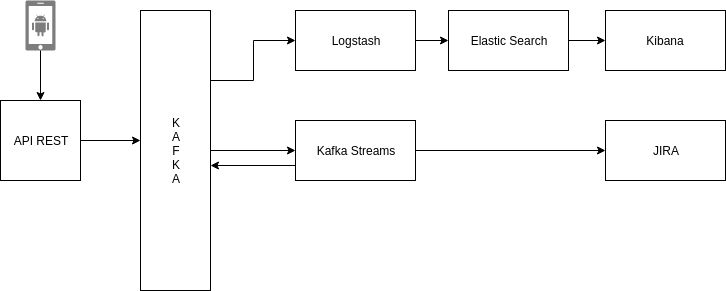
\includegraphics[width=\linewidth]{Arquitectura.png}
	\caption{Arquitectura resultante}
	\label{fig:arquitectura}
\end{figure}
\chapter{Integración de conocimientos}
Los conocimientos que más he integrado en este proyecto son los adquiridos en Redes de Computadores (XC), Internet Móvil (IM), Protocolos de Internet (PI), Seguridad Informática (SI), Proyectos de Tecnologías de la Información (PTI) y Administración de Sistemas Operativos (ASO).

PTI me ha ayudado a planificar la parte técnica del proyecto y a tener en cuenta aspectos como la documentación, el uso de sistemas de versiones, el plantear unos objetivos y elaborar una táctica para llevarlos a cabo.

ASO me ha ayudado a administrar las máquinas a la hora de hacer el despliegue, tener en cuenta las versiones de los programas utilizados y a elaborar scripts que automaticen ciertas partes del despliegue.

IM me ha ayudado a comprender la teoría a bajo nivel sobre la transmisión de información que hacen los dispositivos móviles, me ha hecho tener en cuenta ciertos aspectos a la hora de hacer el envío de eventos y me ha inspirado para la recolección de los eventos.

XC y PI me han ayudado a comprender todo el tema de networking del trabajo, XC sobretodo ha ayudado en la parte de definir las subredes del sistema y PI en decidir cual era la mejor opción para el módulo de recepción de eventos, a parte de ayudarme a tener en cuenta temas de redundancia y balanceo de carga.

SI me ha ayudado a tener en cuenta ciertos aspectos sobre la seguridad del proyecto así como inspirarme en la creación del sistema puesto que en la asignatura se estudian sistema que producen alertas.
 %%DONE
\chapter{Identificación de leyes y regulaciones}

Las dos normativas a las cuales este proyecto podría ser sensible de recibir la aplicación es la Ley Orgánica de Protección de Datos de Carácter Personal (LOPD) a nivel estatal y el Reglamento General de Protección de Datos (GDPR) a nivel europeo, pero no a tal proyecto no se le aplican dichas normativas puesto que no se están recogiendo los datos que tales leyes consideran como sensibles.

La LOPD considera datos de carácter personal: cualquier información numérica, alfabética, gráfica, fotográfica, acústica o de cualquier otro tipo concerniente a personas físicas identificadas o identificables.
En ningún caso se está recogiendo información que puede hacer al usuario identificable.

El GDPR considera datos personales todos aquellos que puedan revelar la identidad del usuario. También incluye direcciones IP pero en el presente proyecto no se recogen direcciones IP de los usuarios. %%DONE


\appendix
%% Cap'itulos incluidos despues del comando \appendix aparecen como ap'endices
%% de la tesis.
\chapter{Diagrama de Gantt} \label{cap:ganttanex}

\begin{landscape}
	\begin{figure}
		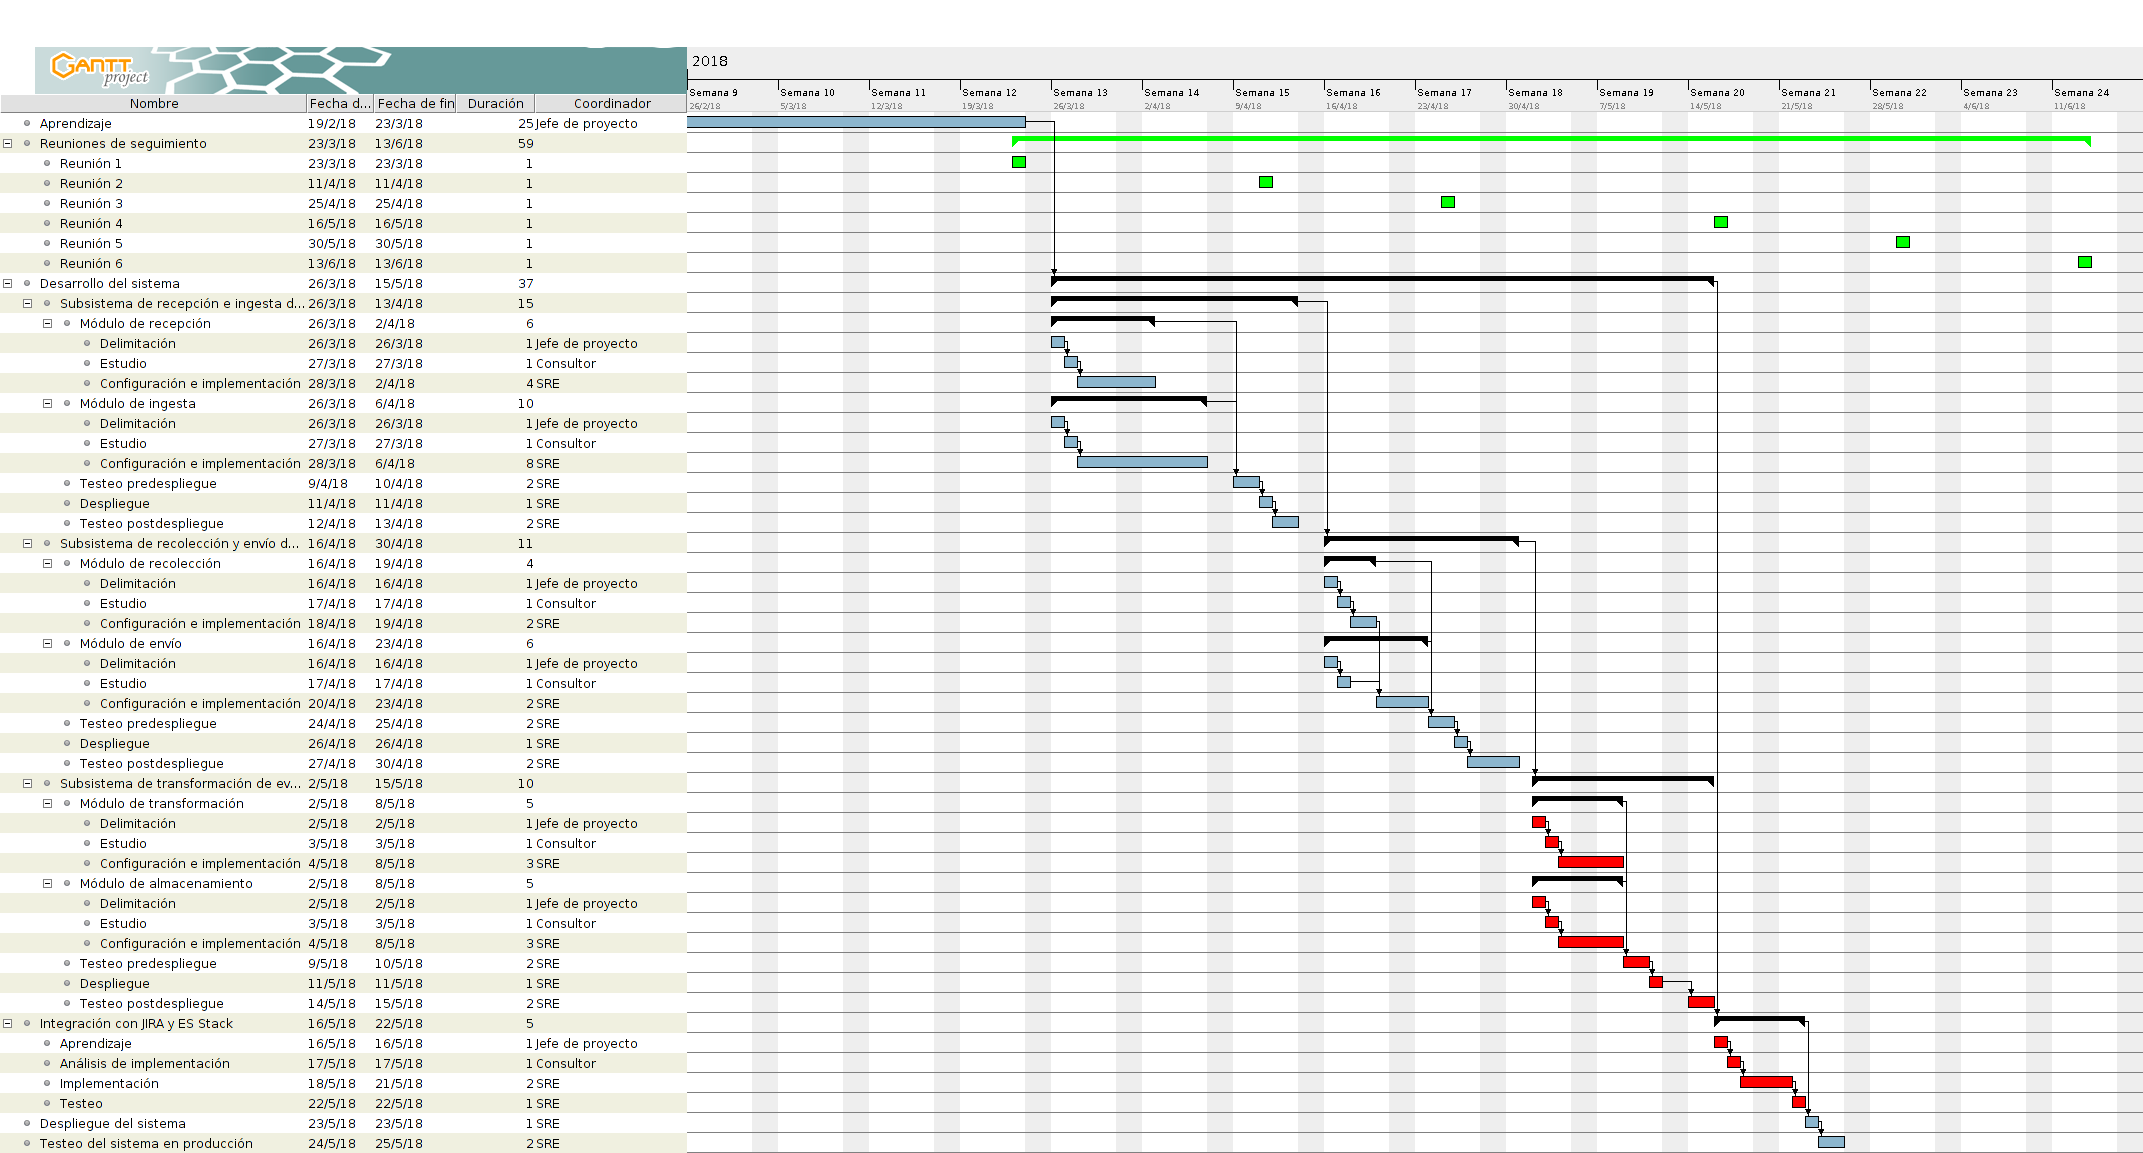
\includegraphics[width=\linewidth]{Gantt.png}
		\caption{Diagrama de Gantt Final}
		\label{fig:gantt}
	\end{figure}
\end{landscape}

\begin{landscape}
	\begin{figure}
		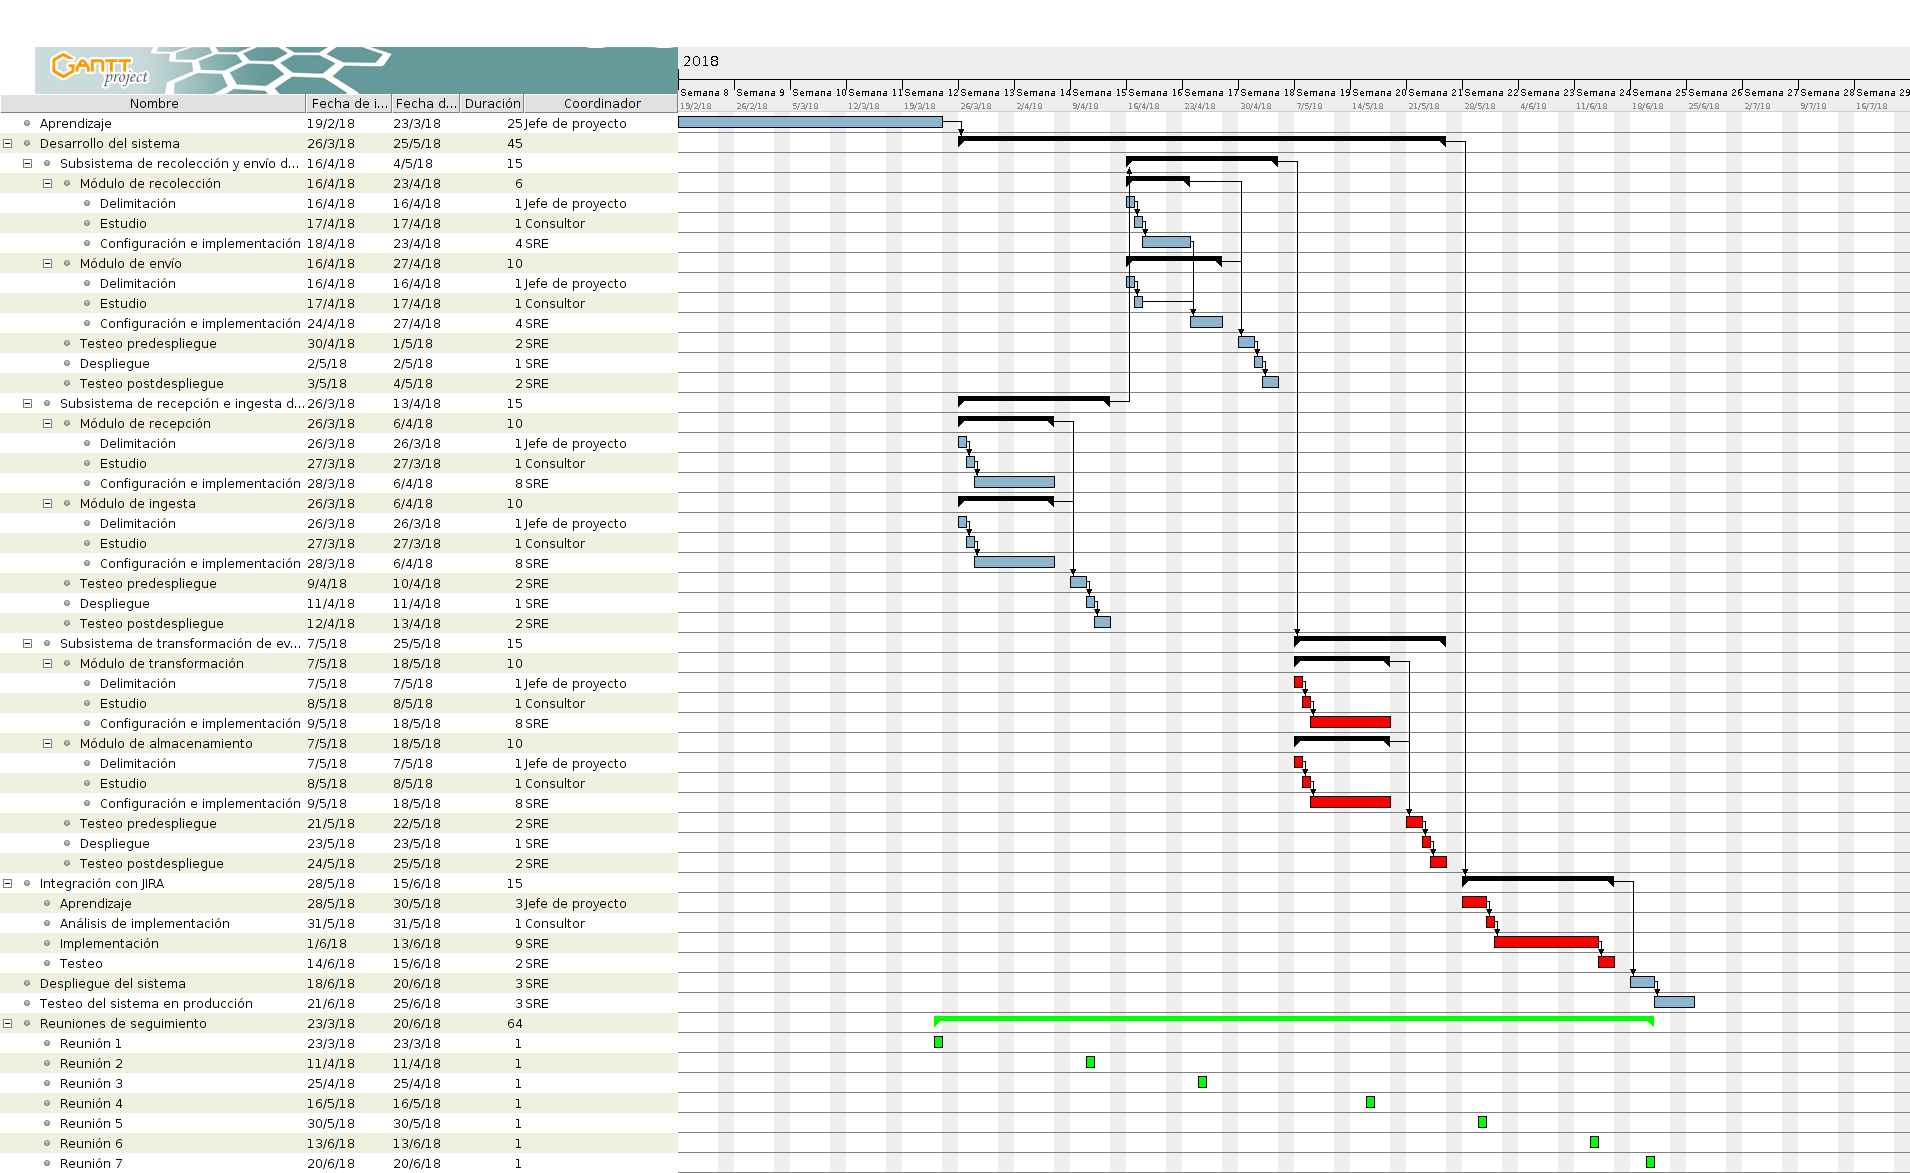
\includegraphics[width=\linewidth]{Gantt_ini.png}
		\caption{Diagrama de Gantt Inicial}
		\label{fig:ganttini}
	\end{figure}
\end{landscape}


%%\chapter{Encuesta conocimientos y competencias en sostenibilidad}
Una vez contestada la encuesta me he dado cuenta de que no he tenido en mente muchos aspectos de sostenibilidad bastante importantes. Por un lado desconocía toda la literatura detrás de la sostenibilidad y los modelos existentes, desconocía el hecho de poder medir cómo de sostenible se es. Mi desconocimiento de la materia en parte puede deberse a que ya llevo años trabajando en la industria y en las empresas que he estado no se ha hecho mucho hincapié en los aspectos de sostenibilidad. Después de haber hecho la encuesta considero que ya empiezo a entender mejor los aspectos que engloba la sostenibilidad y ya empiezo a tenerlos en cuenta en el proyecto, muchos de los aspectos son de sentido común, cosa que puede hacer que se piense que ya se tienen en cuenta cuando se propone un proyecto, pero hay otros aspectos más profundos que es interesante estudiarlos. Por lo que en resumen, mi conocimiento del tema era bastante limitado y me he dado cuenta de que debo de tener en cuenta factores en mi proyecto que pueden ayudar a que este sea sostenible.
Con respecto la calidad de la encuesta, aunque cumple una función de concienciación importante, es mejorable a nivel organizativo. Quizás permitir respuestas más abiertas a las preguntas y organizar las preguntas en subsecciones puede facilitar el hacer resúmenes autoevaluativos posteriormente y darte cuenta qué puntos fuertes y débiles tienes con respecto al tema de la sostenibilidad.
Concluyendo, he de documentarme mejor sobre el tema de la sostenibilidad, no solo porque sea obligación de GEP sino porque es algo importante a nivel social dado que el proyecto tiene un impacto en la sociedad y me he de esforzar de que sea un impacto positivo.
%\include{apendiceB}
%\include{apendiceC}

%% Incluir la bibliograf'ia. Mirar el archivo "biblio.bib" para m'as detales
%% y un ejemplo.
\bibliography{biblio}

\end{document}
